\documentclass[border=5pt]{standalone}
\usepackage{tikz}
\usetikzlibrary{positioning,calc}
\usepackage{fontspec}
\setmainfont{Source Serif 4 Caption}
\begin{document}
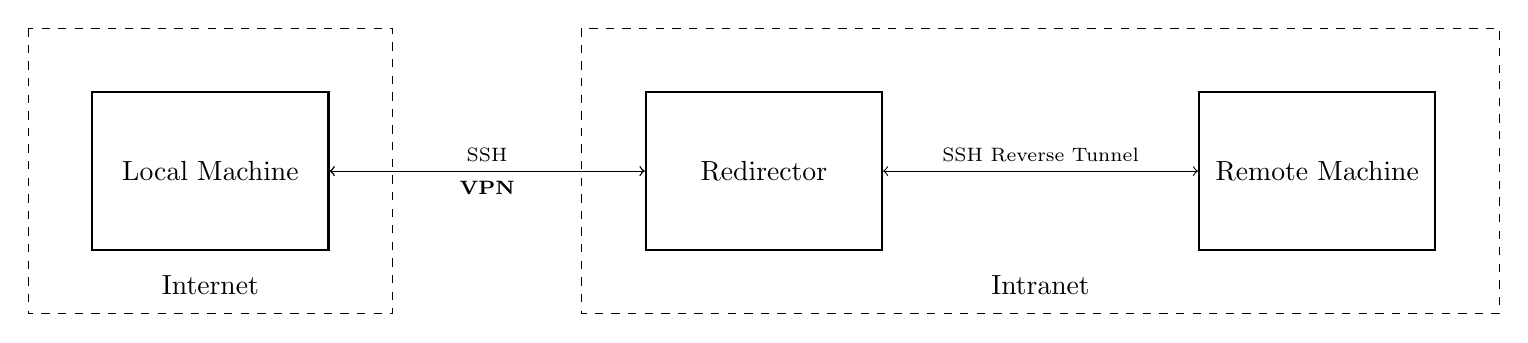
\begin{tikzpicture}[node distance=3cm]
	% Configurable lengths
	\def\connectorLength{1cm}
	\def\networkPadding{0.8cm}
	\def\labelSpacing{1.2cm}

	% Styles
	\tikzstyle{machine}=[draw, rectangle, minimum height=2cm, minimum width=3cm, thick]
	\tikzstyle{arrow}=[->, thick]
	\tikzstyle{label}=[font={\scriptsize}]

	% Machines
	\node[machine] (local) {Local Machine};
	\node[machine, right=of local, xshift=\connectorLength] (redirector) {Redirector};
	\node[machine, right=of redirector, xshift=\connectorLength] (remote) {Remote Machine};

	% Networks
	\draw[dashed] ($(local.north west)+(-\networkPadding,\networkPadding)$) rectangle ($(local.south east)+(\networkPadding,-\networkPadding)$);

	\coordinate (intranet_center) at ($(redirector)!0.5!(remote)$);
	\coordinate (internet_center) at (local.center);

	\draw[dashed] ($(redirector.north west)+(-\networkPadding,\networkPadding)$) rectangle ($(remote.south east)+(\networkPadding,-\networkPadding)$);
	\node[below=\labelSpacing of internet_center] {Internet};
	\node[below=\labelSpacing of intranet_center] {Intranet};

	% VPN Connection
	\draw[<->] (local) -- node[label, below] {\textbf{VPN}} (redirector);
	\draw[<->] (local) -- node[label, above] {SSH} (redirector);

	% Arrows
	\draw[<->] (redirector) -- node[label, above] {SSH Reverse Tunnel} (remote);
\end{tikzpicture}
\end{document}
